\documentclass[dvipdfmx]{beamer}
\usepackage{pxjahyper}
\usepackage{bookmark}
\usepackage{txfonts}

\usetheme{Copenhagen}
\usecolortheme{rose}

\renewcommand{\familydefault}{\sfdefault}
\renewcommand{\kanjifamilydefault}{\gtdefault}

\renewcommand{\figurename}{図}
\renewcommand{\tablename}{表}

\setbeamercovered{dynamic}

\setbeamertemplate{headline}{}
\setbeamertemplate{footline}[page number]
\setbeamertemplate{navigation symbols}{}
\setbeamertemplate{section in toc}[sections numbered]
\setbeamertemplate{items}[default]
\setbeamertemplate{blocks}[rounded]

\usefonttheme{professionalfonts}
\usefonttheme[onlymath]{serif}
\usefonttheme{structurebold}
\setbeamerfont{frametitle}{size=\Large}
\setbeamerfont{title}{size=\Large}

\title{1. FIFO IP Coreとは}
\author{201720690 小松 弘人}
\date{\today}

\begin{document}

\maketitle

\begin{frame}
	\frametitle{Agenda}
	\tableofcontents
\end{frame}

\section{FIFOとは?}
\begin{frame}
	\frametitle{First-In First-Out (FIFO)とは?}
	\begin{itemize}
		\item
			「先入れ先出し」
			\vfill
		\item
			入力された順番にキューから出てくる
	\end{itemize}
	\vfill
	\begin{figure}[ht]
		\centering
		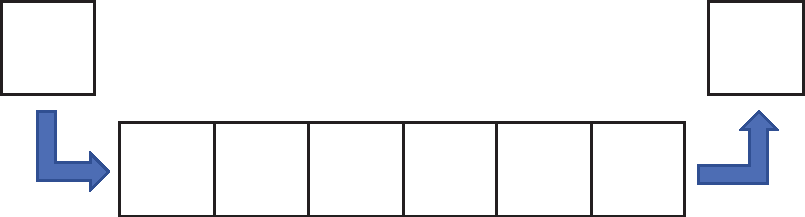
\includegraphics[width=0.6\linewidth]{../img/queue.pdf}
		\caption{First-In First-Out (Queue)}
		\label{img:queue}
	\end{figure}
	\begin{itemize}
		\item
			Vivadoでは、FIFO Generatorを利用してFIFO IP Coreを作る
	\end{itemize}
\end{frame}

\section{FIFOの入出力ポート}
\begin{frame}
	\frametitle{FIFOの入出力ポート}
	\begin{itemize}
		\item
			主な入出力
	\end{itemize}
	\vfill
	\begin{columns}
		\column{.3\textwidth}
			\begin{figure}[ht]
				\centering
				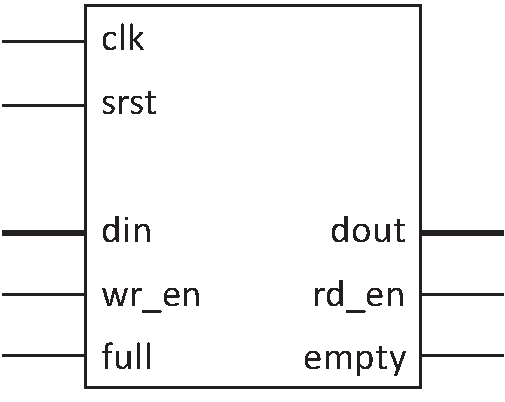
\includegraphics[width=4cm]{../img/fifo_ip.pdf}
				\caption{FIFO IP Core}
				\label{img:fifo_ip}
			\end{figure}
		\column{.7\textwidth}
		\begin{description}
			\item[clk]\mbox{}
				クロック信号
			\item[srst]\mbox{}
				同期リセット信号 (Synchronous ReSeT)
			\item[din]\mbox{}
				データ入力信号
			\item[wr\_en]\mbox{}
				書き込みイネーブル信号
			\item[full]\mbox{}
				FIFOがいっぱいになったらfull=1
			\item[dout]\mbox{}
				データ出力信号
			\item[rd\_en]\mbox{}
				読み出しイネーブル信号
			\item[empty]\mbox{}
				FIFOが空ならempty=1\\
				動作モードで信号が変化
		\end{description}
	\end{columns}
\end{frame}

\section{FIFOの動作モード}
\begin{frame}
	\frametitle{FIFOの動作モード}
	empty信号が1になるタイミングが異なる
	\vfill
	\begin{description}
		\item[Standard mode]\mbox{}
			empty=1になった次のクロックから\\
			データが出力される
		\item[FWFT mode]\mbox{}
			First Word Fall Through (FWFT).\\
			empty=1になったクロックから\\
			データが出力される
	\end{description}
	\vfill
	FWFTモードのFIFOの方が連結しやすい
\end{frame}

\begin{frame}
	\frametitle{シミュレーション波形}
	\begin{figure}[ht]
		\centering
		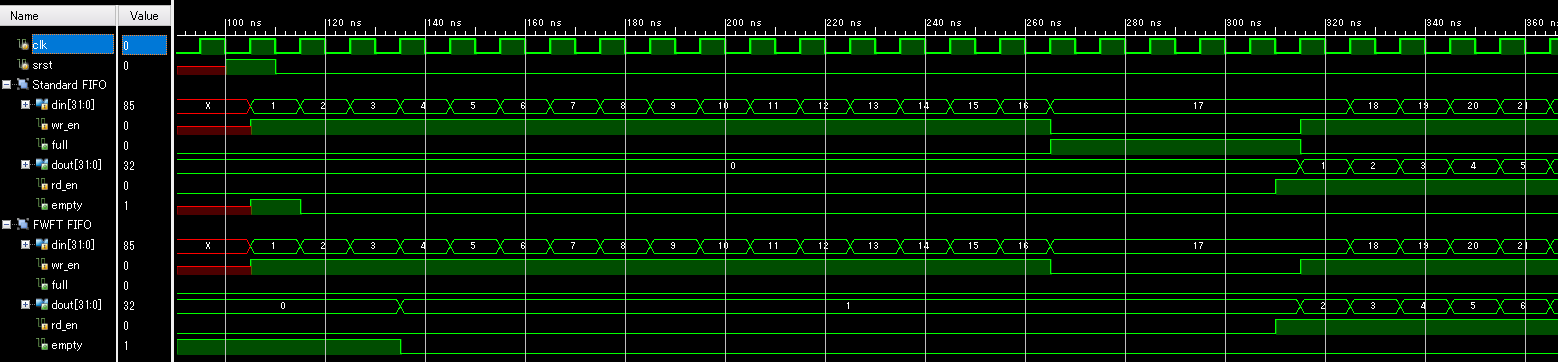
\includegraphics[width=\linewidth]{../img/cmp_fifo.PNG}
		\caption{シミュレーション波形}
			\label{img:cmp_fifo}
	\end{figure}
\end{frame}

\setbeamercovered{invisible}
\section{FIFOの連結}
\begin{frame}
	\frametitle{FIFOの連結}
	複数のFIFOを連結し、1つのFIFOが作れる (AR\# 58928)\\
	wr\_en, rd\_enの配線に注意
	\pause
	\begin{figure}[ht]
		\centering
		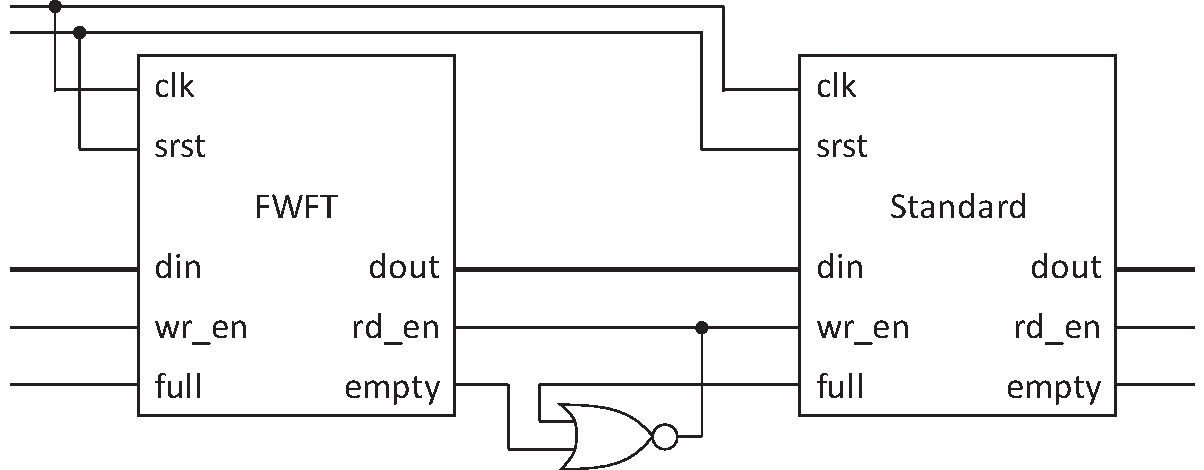
\includegraphics[width=\linewidth]{../img/fifo_join.pdf}
		\caption{FIFOの連結}
		\label{img:fifo_join}
	\end{figure}
\end{frame}
\setbeamercovered{dynamic}

\end{document}
